\documentclass[11pt]{article}
\usepackage{graphicx}
\usepackage{fontspec}


\title{\textbf{Tietokantasovellus: Foorumi}}
\author{Antti Saikkonen}
\date{}

\begin{document}

\maketitle
%Sisällysluettelo!!!
\newpage

\section{Johdanto}
To be added


\newpage
\section{Käyttötapaukset}

\subsection{Käyttötapauskaavio}
\begin{figure}[h]
\centering 
{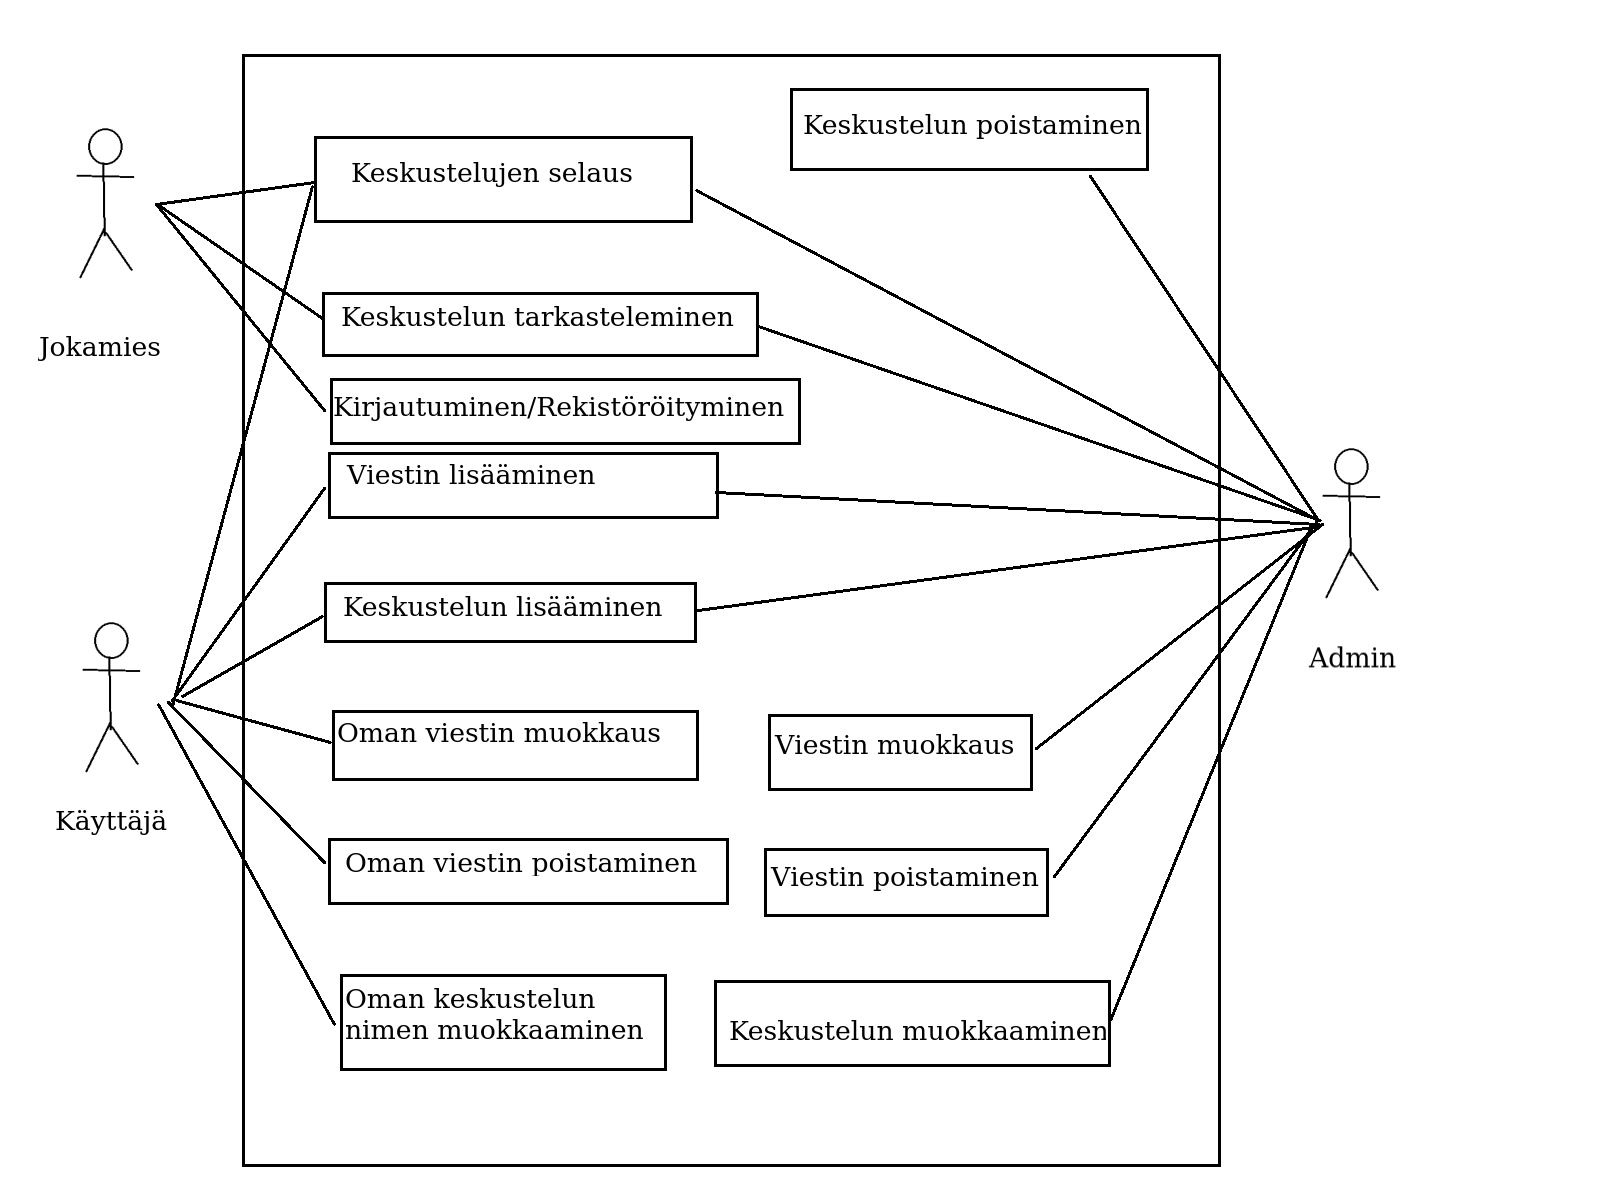
\includegraphics[scale=0.32]{Kayttotapauskaavio.png}}
\caption{Käyttötapauskaavio}
\par
\end{figure}

\subsection{Käyttäjäryhmät}
\textbf{Jokamies}\\
Kuka tahansa sivun käyttäjä.\\\\
\textbf{Käyttäjä}\\
Rekisteröityny käyttäjä.\\\\
\textbf{Admin}\\
Rekisteröitynyt järjestelmänvalvojan oikeuksilla varustettu käyttäjä.


\subsection{Käyttötapaukset}
\textbf{Keskustelujen selaus}\\
Kuka tahansa voi selata listaa keskusteluista, jossa näkyy mm. keskustelun nimi, luoja, aloittamistpäivänmäärä sekä viestien määrä.\\\\
\textbf{Keskustelun tarkasteleminen}\\
Kuka tahansa voi tarkastella keskusteluun lisättyjä viestejä.\\\\
\textbf{Rekisteröityminen/Kirjautuminen}\\
Kuka tahansa voi rekisteröityä palveluun tai kirjautua sisään valmiilla käyttäjätunnuksilla.\\\\
\textbf{Keskustelun lisääminen}\\
Rekisteröitynyt käyttäjä pystyy lisäämään uuden keskustelun.\\\\\
\textbf{Keskustelun muokkaaminen}\\
Rekisteröityneet käyttäjät pystyvät vaihtamaan oman keskustelunsa nimen, admin pystyy muokkaamaan kenen tahansa keskusteluja.\\\\
\textbf{Keskustelun poistaminen}\\
Vain admin pystyy poistamaan keskustelun.\\\\
\textbf{Viestin lisääminen}\\
Rekisteröitynyt käyttäjä pystyy lisäämään viestejä keskusteluihin.\\\\
\textbf{Viestin muokkaus}\\
Rekisteröityneet käyttäjät pystyvät muokkaamaan omia viestejään, admin pystyy muokkaamaan kenen tahansa viestejä.\\\\
\textbf{Viestin poistaminen}\\
Rekisteröityneet käyttäjät pystyvät poistamaan omia viestejään, admin pystyy poistamaan kenen tahansa viestejä.\\\\


\end{document}
